%%%%%%%%%%%%%%%%%%%%%%%%%%%%%%%%%
\section{Production and Quality Assurance}
\label{sec:dp-tpcelec-production}

The \dword{dp} \dword{tpc} electronics system relies on commercially available products as well as custom made electronics elements. The \dword{qc} of the former will be done by the manufacturer, while production and any necessary \dword{qc} of the latter will be ensured by the consortium institutions. 


%%%%%%%%%%%%%%%%%%%%%%%%%%%%%%%%%
\subsection{Charge Readout Electronics}
\label{ssec:dp-tpcelec-prod-cro}

We plan to split production of the front-end analog and digital electronics among several sites in France and Japan. The delivered cards will be divided among institutions in France, Japan, and the USA, where they will be tested and calibrated. Each card test site will be equipped to do \dword{qc} and \dword{qa} checks as well as perform calibration of analog and digital cards. A common database will be developed and populated with test results. 

\begin{dunefigure}[Configuration for QC and calibration of \dshort{cro} electronics system]{fig:dp-tpcelec-qc-chain}
{Overview of the configuration for quality control and calibration of \dword{cro} electronics system.}
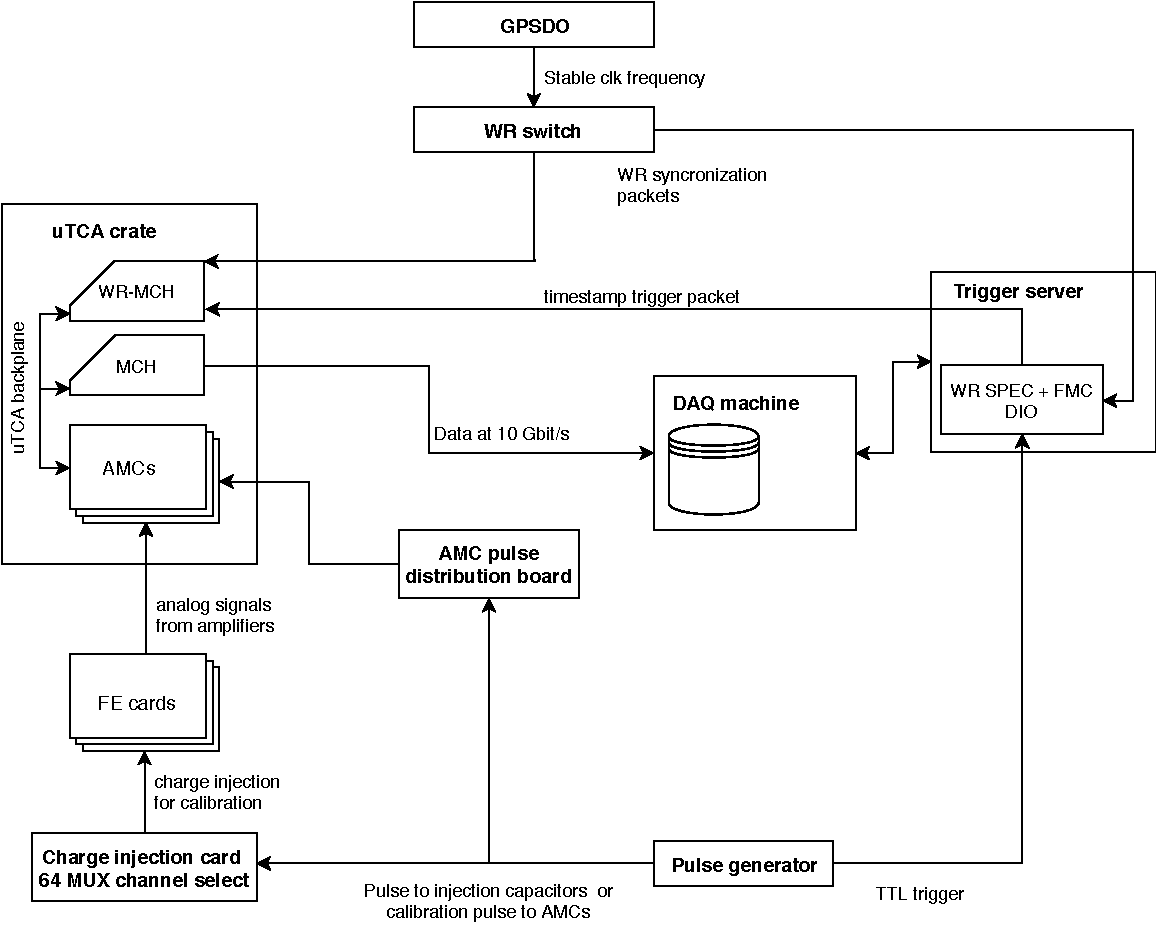
\includegraphics[width=0.8\textwidth]{dp-tpcelec-qc-chain}
\end{dunefigure}


Using the experience with producing \dword{cro} readout electronics for \dword{pddp}, Figure~\ref{fig:dp-tpcelec-qc-chain} schematically illustrates the necessary equipment and set up for the \dword{qc} of both production and calibration. A \dword{utca} crate equipped with \dword{mch} and \dword{wrmch} will host \dwords{amc} to be tested and calibrated. Triggering follows the same scheme as in \dword{pddp} relying on the distribution of timestamped trigger packets over the \dword{wr} network to \dwords{amc}. The triggers are generated by a high precision pulse generator synchronously with the calibration pulse signals sent to the analog or digital electronics.  

Five institutions (IPNL in France; KEK, NITKC, and IU in Japan; and SMU in the USA) share testing responsibilities for the cryogenic \dword{fe} analog cards. The cards will be shipped to each testing site where collaborators will check, at both room and operating cold temperature, performance parameters such as noise levels, dead channels, hot channels, and gain and its uniformity across channels. A dedicated calibration card has been developed, which injects via a precision capacitor a known amount of charge into individual \dword{asic} channels to verify their functionality and calibrate the gain of the amplifiers. The channels selection is automatically performed via a multiplexer.

\begin{dunefigure}[Channel-to-channel gain uniformity on \dshort{fe} cards for \dshort{pddp}]{fig:dp-tpcelec-fec-calib}
{Channel-to-channel gain uniformity measured on \dword{fe} cards produced for \dword{pddp}. The plot on the left illustrates the gain (in units of pulse integral per unit of injected charge) as a function channel number for all the tested cards, while that on the right shows the overall distribution of the gain values fitted to the Gaussian function.}
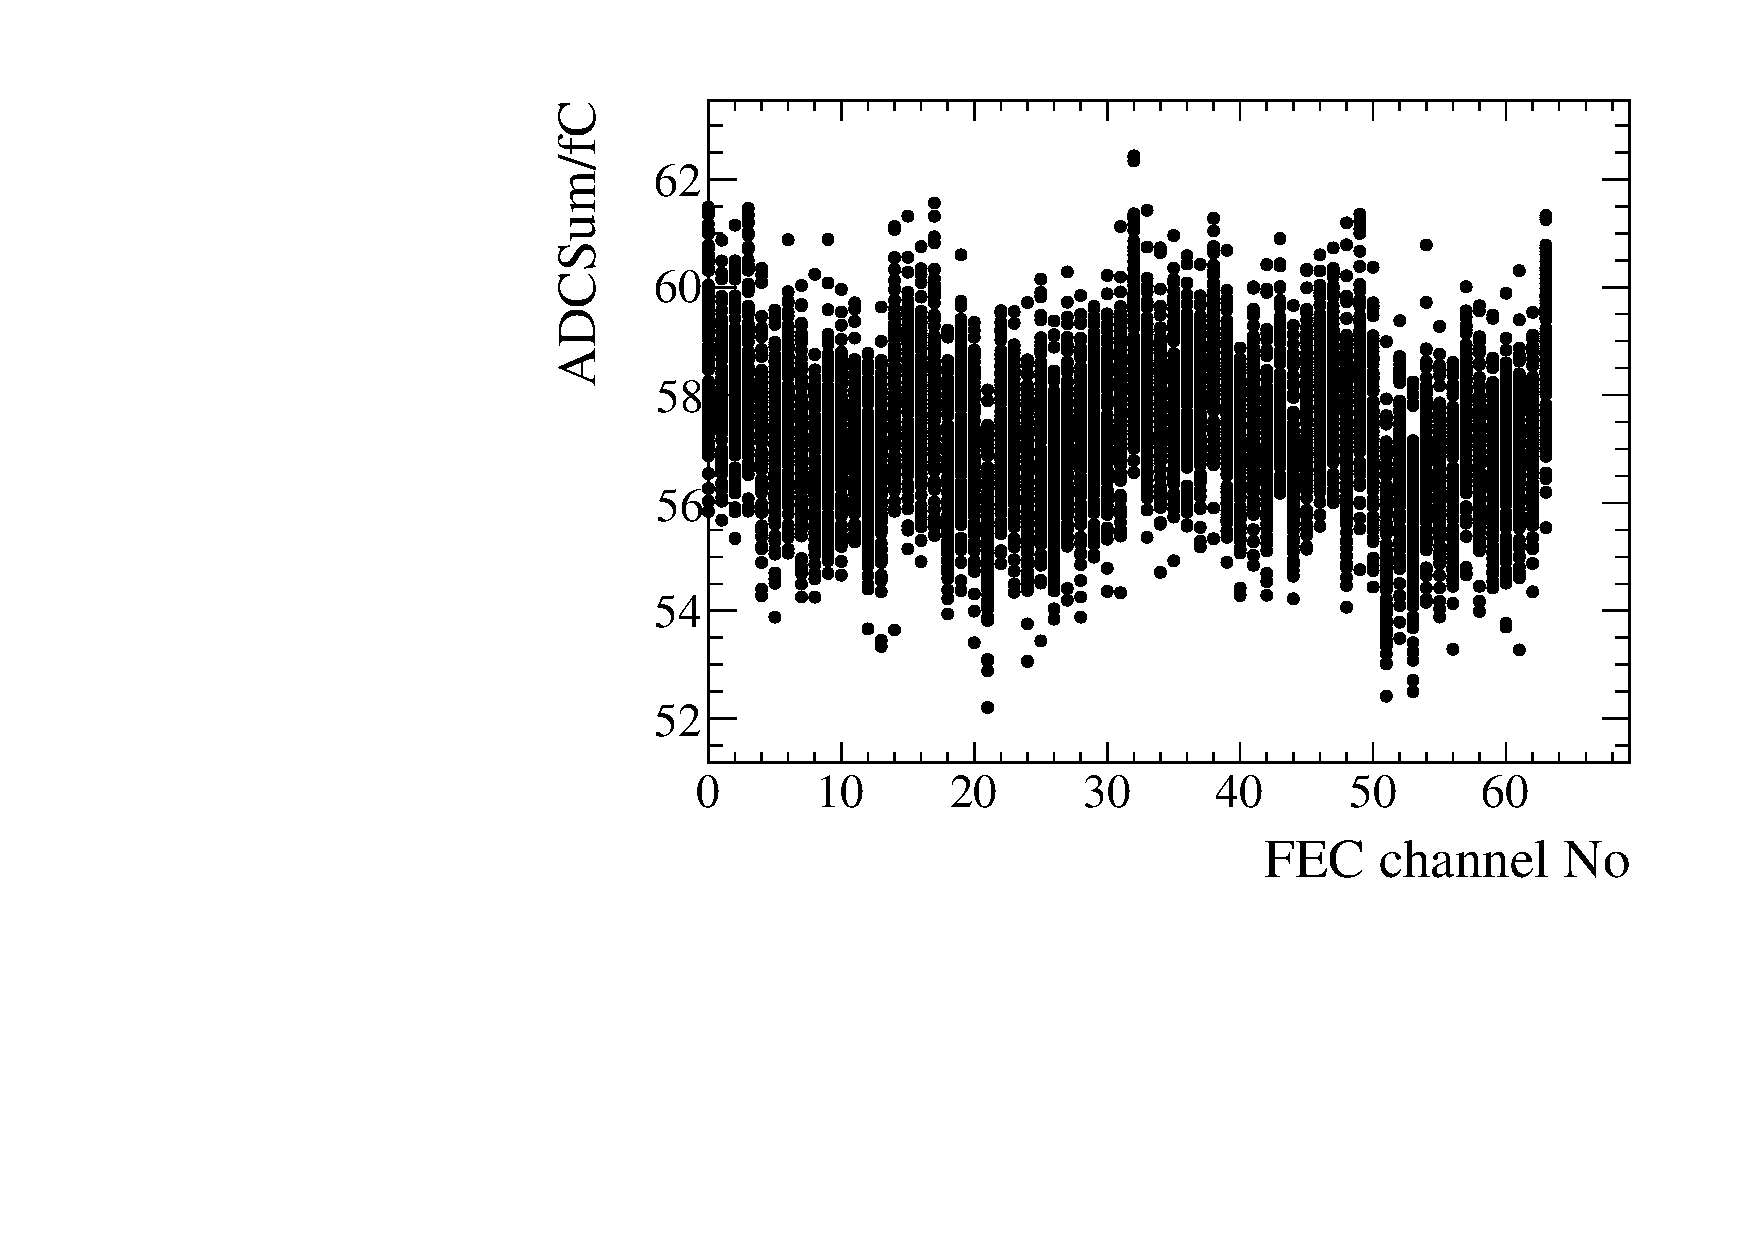
\includegraphics[width=0.45\textwidth]{dp-tpcelec-fec-calib-chnum}
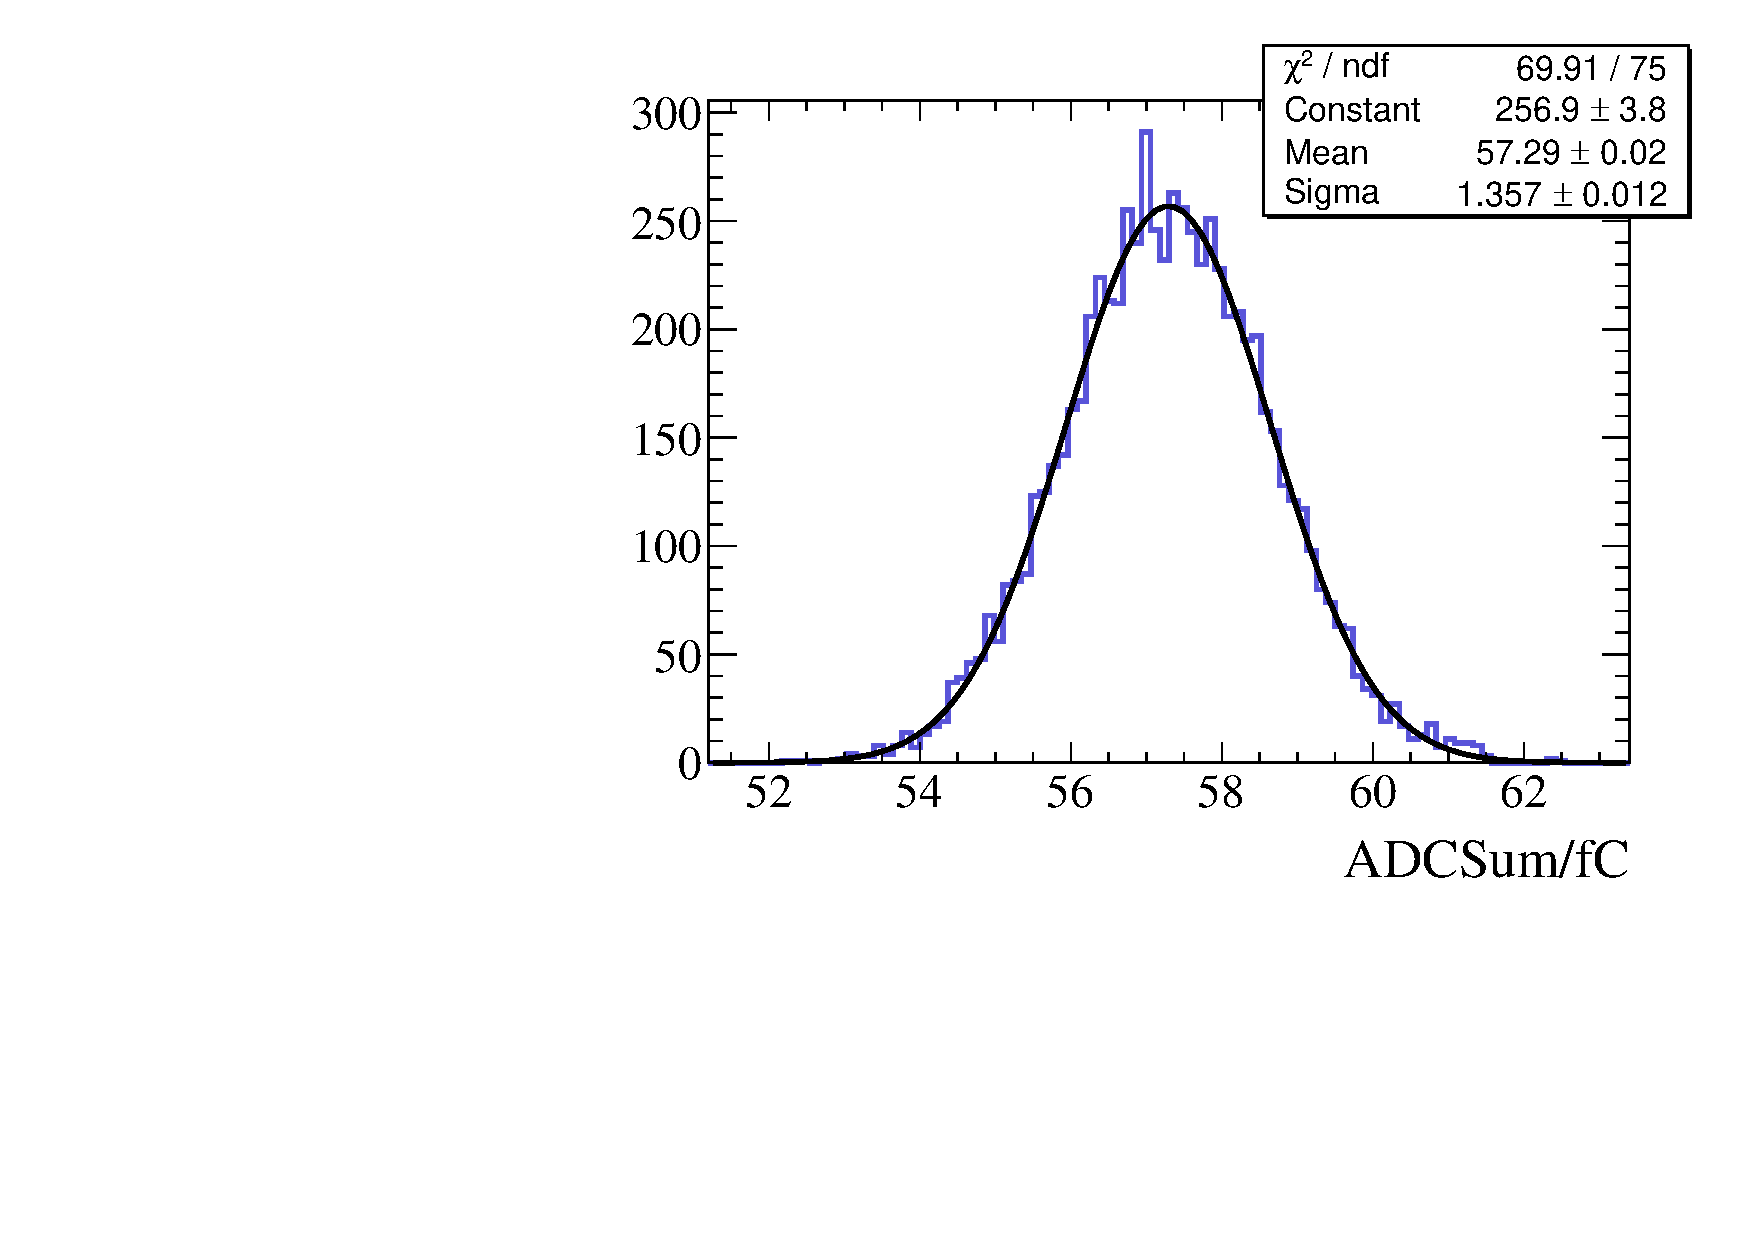
\includegraphics[width=0.45\textwidth]{dp-tpcelec-fec-calib-adcsum}
\end{dunefigure}

As an example, Figure~\ref{fig:dp-tpcelec-fec-calib} illustrates the channel-to-channel gain uniformity from the measurements performed with the \dword{fe} cards produced for \dword{pddp}. The figure on the left shows the gain (in units of pulse integral per unit of injected charge) as a function of channel number for all the cards tested, while that on the right shows the resulting distribution. The small systematic variations in the gain visible in the left-hand plot arise from channel-to-channel variations in the injection card used for calibrating the \dword{fe} amplifiers. Overall, the gain uniformity for all the channels is at \SI{2}{\percent}.

Production of the \dword{amc} cards for the charge readout is currently shared among four institutions (IPNL, KEK, NITKC, and IU). 
The cards ordered and delivered to each of these four institution are subjected to \dword{qc} tests agreed upon by all participants. 

The functionality of \dwords{amc} could be verified by performing acquisition of the pedestal data. In the case of \dword{pddp} production, this test allowed us to identify all the problems in the cards, almost all of which were a result of defective soldering not spotted by the automated \dword{qc} procedure of the manufacturer. To calibrate the \dword{adc} buffer of the \dword{cro} \dwords{amc}, we inject a known pulse (Figure~\ref{fig:dp-tpcelec-qc-chain}) into the input stage and measure the resulting pulse height after digitization. 


%%%%%%%%%%%%%%%%%%%%%%%%%%%%%%%%%  
\subsection{Light Readout Electronics}
\label{ssec:dp-tpcelec-prod-lro}


The number of \dword{lro} \dword{amc} cards required is small enough for production to follow production procedures for \dword{pddp}.
The electronic components of the cards, which meet the required specifications, are purchased commercially. This part of the project will be managed by a qualified engineer working with a specialist in \dword{qa}.

The cards are delivered to designated consortium institutions. Upon delivery, teams conduct basic quality tests, including visual inspection and electrical testing, to ensure conformity of production. Another series of tests will ensure the  % function 
correct %ly 
functionality of the cards and evaluate their performance. Measurements include linearity measurements of each \dword{adc} channel and linearity of the response of the \dword{asic}. The level of cross-talk on the \dword{asic} is also quantified. 

A dedicated single-channel set up, with a \dword{pmt} (Hamamatsu R5912-02-mod) and identical cabling and splitter as in the \dword{dpmod}, can be used to characterize the expected noise level of each channel and the response to single \phel{}s, up to saturation. 
%Several cards operate in each \dword{utca} crate with \dword{daq}. \fixme{last sentence not clear to me} JD - me neither

After shipment to \dword{surf} and on-site installation, a series of tests with a pulse generator will verify that the cards are in good working condition. Noise-level measurements are also included during integration.


%%%%%%%%%%%%%%%%%%%%%%%%%%%%%%%%%
\subsection{Timing System and $\mu$TCA}
\label{ssec:dp-tpcelec-prod-utca}

Production of the cards and procurement of necessary \dword{wr} components for \dword{wrmch} units will be performed by four consortium institutions (IPNL, KEK, NITKC, and IU). The \dword{qc} procedure for \dword{wrmch} cards consists of 
\begin{itemize}
\item{checking the alignment of \dword{pps} signals between the \dword{wr} switch acting as the network grand master (Figure~\ref{fig:dp-tpcelec-qc-chain}) and each \dword{wrmch} slave node, and }
\item{performing data acquisition with functioning \dwords{amc} and verifying the quality of collected data.}
\end{itemize}

The  \num{16} \dword{wr} switches and the \num{245} \dword{utca} crates containing the power modules, carrier hubs (\dword{mch}), and fan units are commercial products. The manufacturer is responsible for the necessary \dword{qa} and \dword{qc}  of these components, requiring no further testing on the part of the \dword{dp} electronics consortium. Once the components are delivered to the designated institutions, they can be sent to \dword{surf} for installation. 


%%%%%%%%%%%%%%%%%%%%%%%%%%%%%%%%%
\subsection{Signal Feedthrough Chimneys}
\label{ssec:dp-tpcelec-prod-sft}

The LAL laboratory will produce the \dwords{sftchimney} and do the \dword{qc}. Led by R. Marie, LAL has invested much engineering effort in the past six months to optimize technical aspects of the design to minimize costs and simplify the production process.

A number of items must be manufactured to produce the \dwords{sftchimney}. These include 
\begin{itemize}
\item PCB flanges for the warm and cold \fdth flange interfaces, 
\item the stainless steel pipe structure, 
\item flanges containing the interfaces to the gas and liquid lines and slow control, 
\item blades and railing, and 
\item the heat exchanger system. 
\end{itemize}
The flat cables that connect the \dword{fe} cards to the warm flange are commercially available products and part of the \dword{sftchimney} procurement process. 

The manufactured components are delivered to designated institutions participating in the \dword{dp} electronics consortium where teams verify signal continuity for both cold and warm flanges, then assemble the components into \dwords{sftchimney} and test for leaks. They also check blade insertion and test flat cables. They pack the assembled \dwords{sftchimney} after verification and ship them to \dword{surf}. 

The commercial VHDCI signal cables (connecting the \dwords{amc} to the \dwords{sftchimney}) are procured and tested with the \dword{sftchimney} warm flanges.


